\section{\ShuffleSnap}
\label{sec:method}

\begin{figure}[tbp]
  \centering
  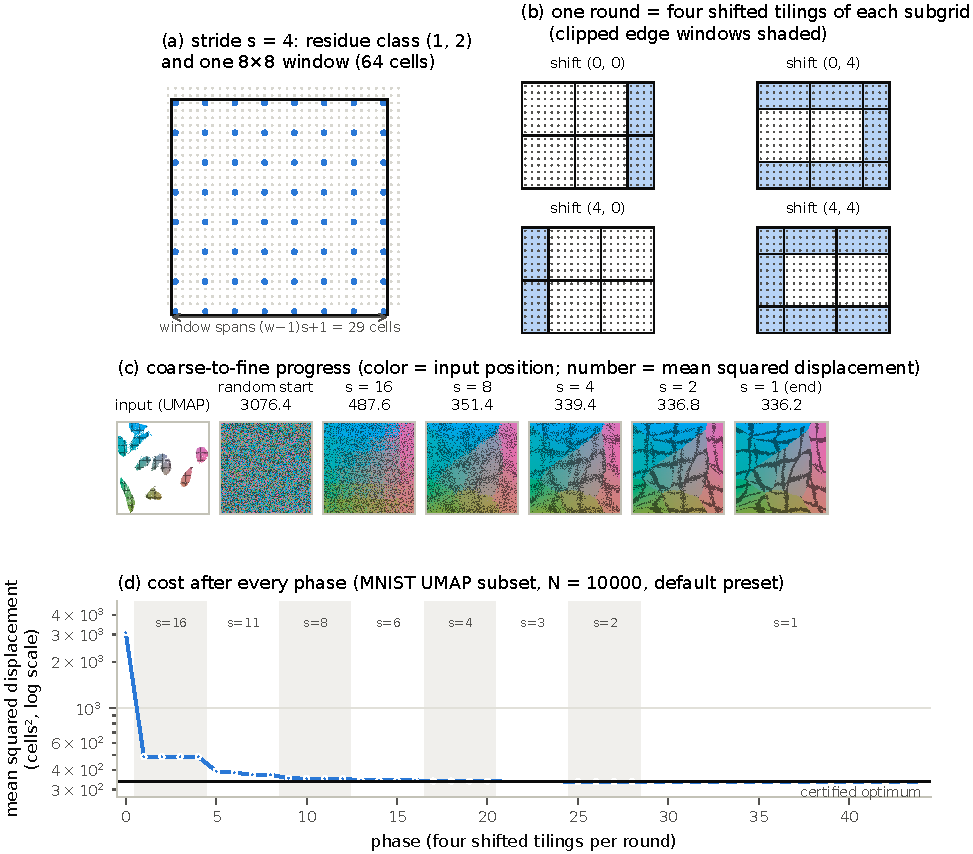
\includegraphics[width=\linewidth]{figures/fig_method.pdf}
  \caption{How \ShuffleSnap\ works. (a)~At stride $s=4$ the lattice splits into
  $s^2=16$ interleaved residue subgrids. Blue marks one of them. An $8\times8$ window of
  that subgrid (filled blue) holds 64 cells spaced 4 apart and spans 29 cells. The
  occupants of those 64 cells are reassigned among the same cells by an exact linear
  assignment. (b)~Each round tiles every subgrid four times, with the tiling shifted by
  half a window in $x$, $y$, or both, so that window borders move. Windows that cross the
  subgrid edge are clipped (shaded), never dropped, on all four sides. (c)~Progress on a
  10{,}000-point subset of a UMAP embedding of MNIST. Each point is colored by its
  \emph{input} position, and the dark bands are the lines of a square grid drawn on the
  input (graph paper). Both travel with the points, so a smooth color field and unbroken
  lines mean the input neighbourhood structure survived; every second stride is shown.
  (d)~Mean squared displacement after every phase. The coarse strides remove most of the
  cost; the stride-1 rounds that follow change little.}
  \label{fig:method}
\end{figure}

\subsection{The algorithm}
\label{sec:algorithm}

\ShuffleSnap\ has two main parameters, the window side $w$ and the stride ratio $r$. The
default is $w=8$ and $r=\sqrt2$ (Section~\ref{sec:improve}).
\begin{enumerate}
\item \textbf{Start.} Place the $N$ points on a uniformly random subset of $N$ cells, as a
  seeded random permutation.
\item \textbf{Strided windows.} At stride $(s_x,s_y)$, lattice positions with the same
  residues $(x \bmod s_x,\, y\bmod s_y)$ form a subgrid, for $s_x s_y$ subgrids in
  total. In its own coordinates each subgrid is tiled with $w\times w$ windows. A window
  therefore contains at most $w^2$ cells (64 by default), spaced $s$ apart on the lattice
  and spanning $(w-1)s+1$ cells per axis.
\item \textbf{Exact reassignment.} In every window, the points currently occupying its
  cells are reassigned among the same cells, empty ones included, by solving the dense
  linear assignment on squared distances to the original (normalized) coordinates. The
  window's cell set never changes, so the global assignment stays injective.
\item \textbf{Shifted tilings.} The tiling is repeated with shifts $(0,0)$, $(0,w/2)$,
  $(w/2,0)$ and $(w/2,w/2)$ in subgrid coordinates. These four phases form one round.
  Windows in one phase are disjoint and are solved in parallel.
\item \textbf{Schedule.} On an axis of length $L$, the first stride is the smallest power of
  two with $ws\ge L$, so that the first windows span the grid. After one round, both strides
  are divided by $r$ and rounded, with repeats removed and never below 1. Stride-1 rounds
  then repeat until a full round moves no point, or until a time budget runs out.
\end{enumerate}
With $r=2$ the strides halve, and every level quarters the area a window spans. With
$r=\sqrt2$ the area halves from one level to the next, so each level starts from a layout
that is already sorted at nearly its own scale; this plausibly explains why $\sqrt2$ works
well (Section~\ref{sec:ablation}). It roughly doubles the number of levels.

\paragraph{Window solver and acceptance.} Each window is a rectangular problem: $k$
occupants and $m\ge k$ cells, with $m\le w^2$. We solve it exactly by
shortest augmenting paths with dual potentials (the Hungarian method, $O(k^2m)$ time),
started from duals built from the window's geometry (Section~\ref{sec:geosolver}). A new window assignment replaces the old
one only if it is cheaper by more than a relative $10^{-12}$. Because the old assignment
is feasible for the window problem, every accepted change strictly lowers the global
cost by at least that margin. Hence the cost sequence is monotone, the search
terminates, and ties (e.g.\ duplicated points) never cause cycling.

\subsection{A geometric window solver}
\label{sec:geosolver}

Almost all of the running time is spent in window solves, so the choice of solver matters. Generic
LAP solvers are slow on these windows for a geometric reason. On clustered data, and at
coarse strides in particular, a window's occupants often come from a dense cluster that
lies far from most of the window's cells. Seen from far away, every point prefers the same
corner cell. The usual greedy start (match each row to its cheapest free column) then
matches little, and the shortest augmenting paths become long. We captured about
79{,}000 windows from runs with $8\times8$ windows and $r=\sqrt2$ (20{,}000 points; unchanged
windows skipped as in the kernel). In 96\% of the MNIST windows with at least 16 points, the
points' cheapest cells numbered at most half as many as the points (median: one cheapest
cell per 3.6 points). On uniform points this happened in 1\% of the windows.

The squared-distance structure offers a better start. For the cost $|p-q|^2$, optimal
duals on the cells are a discretized Brenier potential~\citep{brenier1991polar}: $v(q)=|q|^2-2\psi(q)$ with $\psi$
convex, and $\nabla\psi$ maps cells to the points that occupy them. We use the potential
of a map that is optimal per axis. On one axis, the optimal transport between the points'
and the cells' coordinates is the sorted order, and its potential is piecewise linear:
between consecutive distinct cell coordinates, $\psi$ increases at a rate equal to the
point quantile at that cumulative cell mass. Summing the two axes gives separable starting
duals in $O(k\log k+m\log m)$ time. They move a distant cluster onto the window and
spread it over the window's rows and columns, which removes most of the conflicts. The
solver then proceeds in four exact steps:
\begin{enumerate}
\item row reduction under the starting duals, and a greedy match of every row whose
  cheapest column is still free;
\item a column reduction, which keeps the duals feasible and makes every cell tight for at
  least one point;
\item Kuhn's augmenting paths restricted to tight (zero reduced cost) edges, for the rows
  still unmatched;
\item shortest augmenting paths for the rest (Dijkstra over a shrinking list of unscanned
  columns with lazy dual updates, ties broken towards free columns, as in
  SciPy's solver~\citep{crouse2016implementing}).
\end{enumerate}
Arbitrary starting duals are valid only for a square problem. A window with empty cells is
therefore either padded with zero-cost rows and solved from the geometric start, or, if
fewer than half of its rows compete for a cell under zero duals (as on near-uniform data),
solved directly as a rectangular problem from zero duals. Padding such a window would cost
one augmenting path per empty cell.

On the captured windows, the solver returned the optimum on every window. It was 5.1--5.6$\times$ faster
than the Hungarian method with a greedy start on MNIST and mixture windows, and
1.9$\times$ faster on uniform ones. In full runs with the default $8\times8$ windows it is
5.1--5.3$\times$ faster on clustered inputs and 2.0--2.1$\times$ faster on uniform points, on 1
or 24 threads (Section~\ref{sec:ablation}). Its results are identical to the other exact
solvers' up to ties.
\subsection{Implementation}
\label{sec:impl}

The kernel is C++17, exposed to Python with nanobind, and parallelized with OpenMP over
the windows of a phase. Each thread keeps its own scratch buffers. Because windows in a
phase are disjoint and each solve is deterministic, the result is bit-identical for any
thread count; a test checks this. We also track, for every cell, the last phase that
changed its occupant. A window whose cells are unchanged since it was last solved in the
same stage is already optimal, and skipping it does not change the result (also tested).
This matters in the stride-1 convergence rounds, where most windows are untouched. The
cost is recomputed exactly after every phase, which gives an anytime trace, and a time
budget is checked between windows. A serial reference of about 70 lines of NumPy and SciPy
(Appendix~\ref{app:reference}) returns exactly the kernel's assignments and serves as an
executable specification. There is no just-in-time compilation, so nothing is compiled at run time. Compiling the
extension takes 2.6\,s with parallel Ninja (8.1\,s on one core). A complete isolated wheel
build, including creating the build environment as \texttt{pip install} does from source,
takes about 35\,s.

\paragraph{Work per level.} A phase at stride $s$ has about $M/w^2$ windows (plus clipped
ones), each an $O(w^6)$ Hungarian solve in the worst case. The work per phase is
therefore $O(Mw^4)$, independent of $s$, and a schedule with $\ell$ levels costs
$O(\ell M w^4)$ plus the convergence rounds. With $\ell=O(\log L)$ this is
$O(M\log M)$ for fixed $w$. The constant depends strongly on the data: windows far from
optimal need long augmenting paths.

\subsection{Choosing the parameters}
\label{sec:improve}

We chose every setting on a development set (instance seed 0: 23 instances of 10{,}000 to
100{,}000 points, including masks and surplus cells, five start seeds each) and report
every claim on held-out seeds (Section~\ref{sec:ablation}).

\begin{itemize}
\item \textbf{Window size} is the main quality knob. We tried window sides from 6 to 24
  with four stride ratios (35 configurations). Every step up in window size lowered the
  excess, and the gains did not level off: from $8\times8$ to $12\times12$ to $16\times16$
  windows, each step cost 2--2.6 times the time and removed one half to two thirds of the
  remaining excess. There is no sweet spot, so we place three presets along the curve, two of
  them where they can be compared with BSP-OT at equal time: \emph{fast} ($5\times5$ windows)
  takes about as long as BSP-OT with 16 plans, its default, and \emph{balanced} ($8\times8$,
  our default) about as long as BSP-OT with 64 plans, on one core at $10^5$ points.
  \emph{Quality} ($12\times12$) is one step further. For the fast preset, $5\times5$ windows
  with ratio $\sqrt2$ beat $6\times6$ windows with halving strides, which take the same time,
  on five of seven development instances. Windows up to $32\times32$ can be set explicitly. The cost of a window
  solve grows as $w^6$ in the worst case, but a phase has $M/w^2$ windows and most of them
  are nearly sorted or skipped; in our runs the total time grew as about $w^{1.9}$ (uniform)
  to $w^{2.8}$ (clustered data). Using small windows at coarse strides and large ones at
  stride 1 was worse than using large windows throughout.
\item \textbf{Stride ratio.} Dividing strides by $\sqrt2$ instead of 2 (rounded, duplicates
  removed) roughly doubles the number of levels, each at about the same cost, and was on
  or next to the best time--quality trade-off at every window size. Ratios of 1.68 and
  1.19 were close; 2 and 3 were clearly worse.
\item \textbf{Start.} Structured starts are mostly \emph{worse} than a random
  permutation: bisection (the recursive median split used by RasterFairy-like methods) on
  every input, and row sorting on most. They create straight seams that the local windows
  cannot repair. The random start is a decorrelating device, not a lazy default.
\item \textbf{Solver.} All solvers we tried are exact, so they change only time. JV with
  augmenting row reduction is slower than the Hungarian method on these windows,
  because squared distances create many near-ties. An $\varepsilon$-scaled auction whose
  prices warm-start the same exact shortest-path finish is 2--3$\times$ faster on clustered
  data but not on uniform points. The geometric solver (Section~\ref{sec:geosolver}) is the
  fastest on every input. Variants that did not pay off, measured on the captured
  windows: starting duals from an affine or a full-covariance Gaussian map (both worse than
  the per-axis quantile map), duals integrated from the current assignment (better on
  clustered windows, worse on uniform ones, and choosing per window cost more than it
  saved), an auction refinement of the geometric start, repeated row and column
  reductions, and a branch-free scan of all columns in the shortest-path step.
\item \textbf{Post-processing.} Extra stride-2 and stride-1 rounds after convergence changed
  nothing on seven of nine held-out instances (a stride-2 window cannot move a point by one
  cell).
  Merging independent runs component by component, the rule BSP-OT uses, helps less per
  unit time than a larger window.
\end{itemize}
